%%
% This is an Overleaf template for presentations
% using the TUM Corporate Desing https://www.tum.de/cd
%
% For further details on how to use the template, take a look at our
% GitLab repository and browse through our test documents
% https://gitlab.lrz.de/latex4ei/tum-templates.
%
% The tumbeamer class is based on the beamer class.
% If you need further customization please consult the beamer class guide
% https://ctan.org/pkg/beamer.
% Additional class options are passed down to the base class.
%
% If you encounter any bugs or undesired behaviour, please raise an issue
% in our GitLab repository
% https://gitlab.lrz.de/latex4ei/tum-templates/issues
% and provide a description and minimal working example of your problem.
%%


\documentclass[
  english,            % define the document language (english, german)
  aspectratio=169,    % define the aspect ratio (169, 43)
  % handout=2on1,       % create handout with multiple slides (2on1, 4on1)
  % partpage=false,     % insert page at beginning of parts (true, false)
  % sectionpage=true,   % insert page at beginning of sections (true, false)
]{tumbeamer}


% load additional packages
\usepackage{booktabs}
% Insert pictures and graphs
\usepackage{graphicx}
\graphicspath{{figures/}}

\usepackage{tikz}
\usetikzlibrary{positioning, calc}
\usepackage{booktabs}
\usepackage{multirow}
\usepackage{array}
\usepackage{ulem}


% presentation metadata
\title{Increasing Reward Quality \& Density for Verifiable Rewards}
\author{Ana Cunha, Leonard Evers, Leonhard Driesch}

\institute{\\\theUniversityName}
\date[06/24/2026]{June 24\textsuperscript{th}, 2026}

\footline{\insertauthor~|~\insertshorttitle~|~\insertshortdate}


% macro to configure the style of the presentation
\TUMbeamersetup{
  title page = TUM tower,         % style of the title page
  part page = TUM toc,            % style of part pages
  section page = TUM toc,         % style of section pages
  content page = TUM more space,  % style of normal content pages
  tower scale = 1.0,              % scaling factor of TUM tower (if used)
  headline = TUM threeliner,      % which variation of headline to use
  footline = TUM default,         % which variation of footline to use
  % configure on which pages headlines and footlines should be printed
  headline on = {title page},
  footline on = {every page, title page=false},
}

% available frame styles for title page, part page, and section page:
% TUM default, TUM tower, TUM centered,
% TUM blue default, TUM blue tower, TUM blue centered,
% TUM shaded default, TUM shaded tower, TUM shaded centered,
% TUM flags
%
% additional frame styles for part page and section page:
% TUM toc
%
% available frame styles for content pages:
% TUM default, TUM more space
%
% available headline options:
% TUM empty, TUM oneliner, TUM twoliner, TUM threeliner, TUM logothreeliner
%
% available footline options:
% TUM empty, TUM default, TUM infoline


\begin{document}

\maketitle

\section{Introduction}

\begin{frame}{Motivation}

\begin{columns}[c]

\begin{column}{0.48\textwidth}
\begin{itemize}
    \item RL for LLMs often suffers from
          \textbf{reward sparsity}.
    \item Particularly severe for
          \textbf{binary verifiable rewards}.
    \item The model receives only a final
          \textbf{0/1 reward}.
    \item Intermediate reasoning steps receive
          no direct feedback.
\end{itemize}
\end{column}

\begin{column}{0.52\textwidth}
\centering
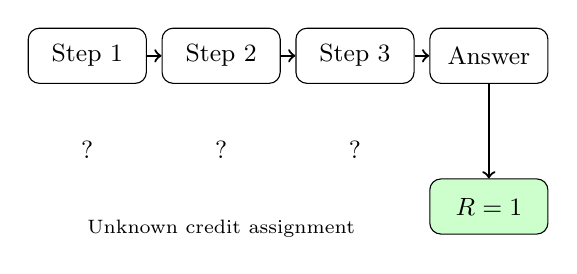
\begin{tikzpicture}[
    node distance=1.7cm,
    every node/.style={font=\small},
    state/.style={
        draw,
        rounded corners,
        minimum width=1.5cm,
        minimum height=0.7cm
    },
    reward/.style={
        draw,
        rounded corners,
        fill=green!20,
        minimum width=1.5cm,
        minimum height=0.7cm
    }
]

\node[state] (s1) {Step 1};
\node[state, right of=s1] (s2) {Step 2};
\node[state, right of=s2] (s3) {Step 3};
\node[state, right of=s3] (s4) {Answer};

\node[reward, below=1.2cm of s4] (r) {$R=1$};

\draw[->, thick] (s1) -- (s2);
\draw[->, thick] (s2) -- (s3);
\draw[->, thick] (s3) -- (s4);
\draw[->, thick] (s4) -- (r);

\node[below=0.6cm of s1] {?};
\node[below=0.6cm of s2] {?};
\node[below=0.6cm of s3] {?};

\node[below=1.6cm of s2, align=center]
{\scriptsize Unknown credit assignment};

\end{tikzpicture}
\end{column}

\end{columns}

\vspace{0.5cm}
\begin{block}{Key Challenge}
How can we identify which intermediate reasoning steps deserve credit when only the final outcome is observed?
\end{block}

\end{frame}

\begin{frame}{Our Approach}

\begin{block}{Goal}
Increase reward density for binary verifiable tasks by identifying
\textbf{critical reasoning steps} within successful trajectories.
\end{block}

\vspace{3mm}

\textbf{Key Idea: Master/Novice Credit Assignment}

\vspace{1mm}

\begin{itemize}
    \item Start from a strong LLM (the \textbf{Master}) and construct a weaker variant (the \textbf{Novice}).
    \item Compare the action probabilities predicted by both models at every reasoning step.
    \item Large divergences indicate steps where the Master uses knowledge or reasoning unavailable to the Novice.
    \item These steps receive higher reward, while agreement corresponds to routine or uninformative transitions.
\end{itemize}

\end{frame}


\begin{frame}{Our Approach}{Master/Novice divergence as a reward signal}

\centering

\begin{tikzpicture}[
    font=\small,
    tok/.style={draw, rounded corners, minimum width=1.2cm, minimum height=0.7cm},
    master/.style={tok, fill=TUMBlue!25},
    novice/.style={tok, fill=TUMBlue!8},
    crit/.style={tok, fill=TUMOrange!30, very thick},
    flow/.style={->, thick, TUMBlue},
    div/.style={<->, thick, TUMOrange},
]

% --- Master track (top): generates the rollout ---
\node[align=center, font=\bfseries] (mlab) at (-0.2, 1.05) {Master\\[-1pt]\scriptsize strong};
\node[master, right=1.1cm of mlab] (m1) {$t_1$};
\node[master, right=0.45cm of m1]  (m2) {$t_2$};
\node[crit,   right=0.45cm of m2]  (m3) {$t_3$};
\node[master, right=0.45cm of m3]  (m4) {ans};

\draw[flow] (m1) -- (m2);
\draw[flow] (m2) -- (m3);
\draw[flow] (m3) -- (m4);
\node[TUMBlue, font=\scriptsize] at ($(m1)!0.5!(m4) + (0,0.62)$) {generates rollout};

% --- Novice track (bottom): re-scores the same tokens ---
\node[align=center, font=\bfseries] (nlab) at (-0.2, -1.05) {Novice\\[-1pt]\scriptsize weak};
\node[novice] (n1) at (m1 |- nlab) {$p_1$};
\node[novice] (n2) at (m2 |- nlab) {$p_2$};
\node[novice] (n3) at (m3 |- nlab) {$p_3$};
\node[novice] (n4) at (m4 |- nlab) {$p_4$};
\node[font=\scriptsize] at ($(n1)!0.5!(n4) + (0,-0.62)$) {re-scores the same tokens};

% --- Divergence between the tracks ---
\draw[div] (m1) -- (n1) node[midway, right, font=\scriptsize] {$\delta_1$};
\draw[div] (m2) -- (n2) node[midway, right, font=\scriptsize] {$\delta_2$};
\draw[div, line width=1.4pt] (m3) -- (n3)
    node[midway, right, font=\scriptsize\bfseries, TUMOrange] {$\delta_3$ large};
\draw[div] (m4) -- (n4) node[midway, right, font=\scriptsize] {$\delta_4$};

\node[align=center, font=\scriptsize, TUMOrange, right=0.3cm of m4, xshift=0.2cm]
    {critical\\token};

\end{tikzpicture}

\vspace{2mm}

\begin{block}{Reward signal}
Large divergence $\delta_t$ \;$\Rightarrow$\; the token relies on knowledge the Novice lacks \;$\Rightarrow$\; higher credit.
\end{block}

\end{frame}


\section{Related Work}

\begin{frame}{Turning Partial Success into Dense Verifiable Rewards}

\textbf{Core problem in code RL}

\begin{itemize}
    \item Verifiable rewards enforce \textbf{correctness via tests}
    \item But they are \textbf{extremely sparse} (only pass/fail)
\end{itemize}

\vspace{2mm}

\textbf{Existing alternatives}


\begin{itemize}
    \item External reward models → dense but \textbf{misaligned + expensive}
\end{itemize}

\vspace{2mm}

\textbf{Key observation}

\begin{center}
Partial test success already exists \;\; $\rightarrow$ \;\; unused signal
\end{center}

\vspace{2mm}

\textbf{Idea}

\begin{block}{Can we use pass rate as a dense reward signal?}
Instead of binary success, use fraction of passing tests as supervision?
\end{block}

\end{frame}

\begin{frame}{Turning Partial Success into Dense Verifiable Rewards}{Answer:}

\centering
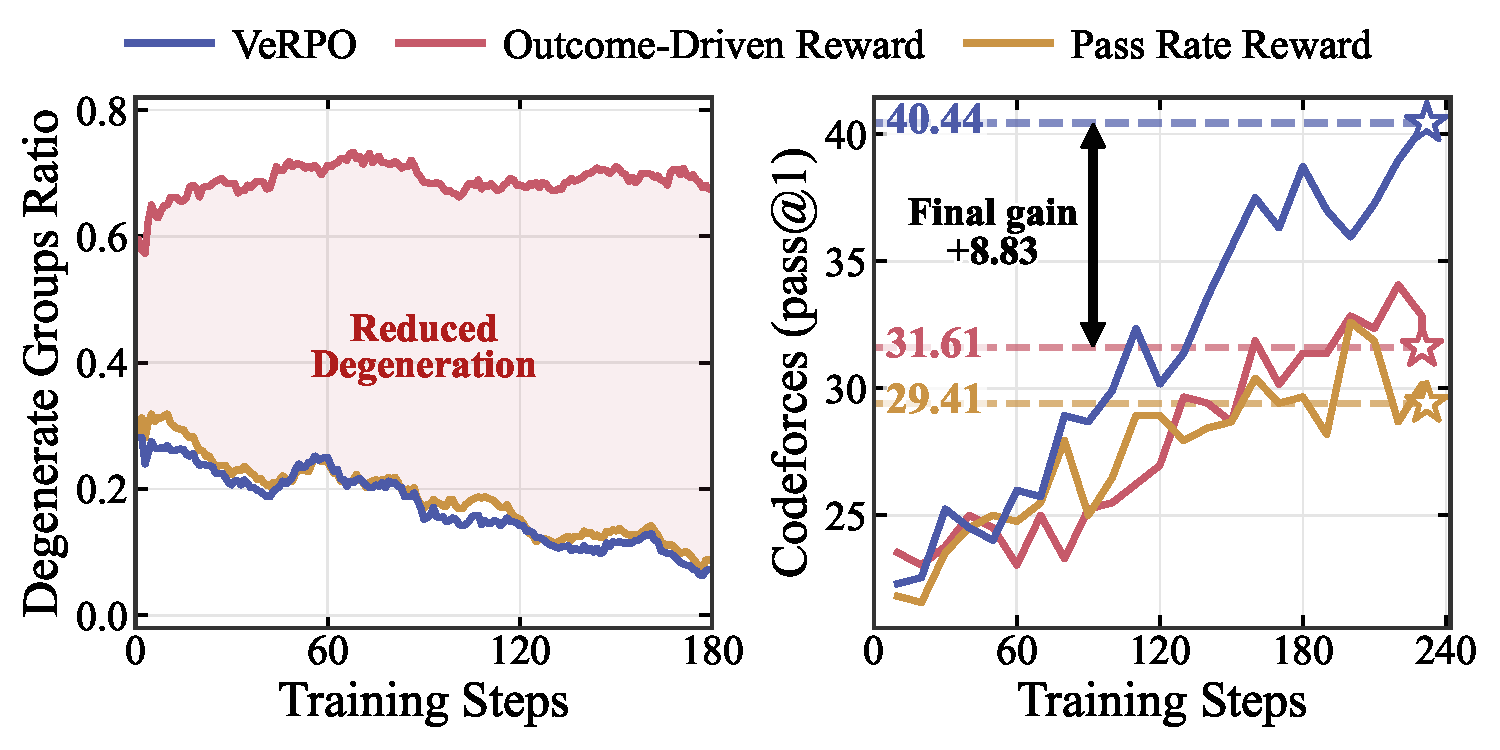
\includegraphics[width=0.8\textwidth]{combined_evaluation_plots_may.pdf}

\end{frame}

\begin{frame}{Turning Partial Success into Dense Verifiable Rewards} {Problem:}

\centering
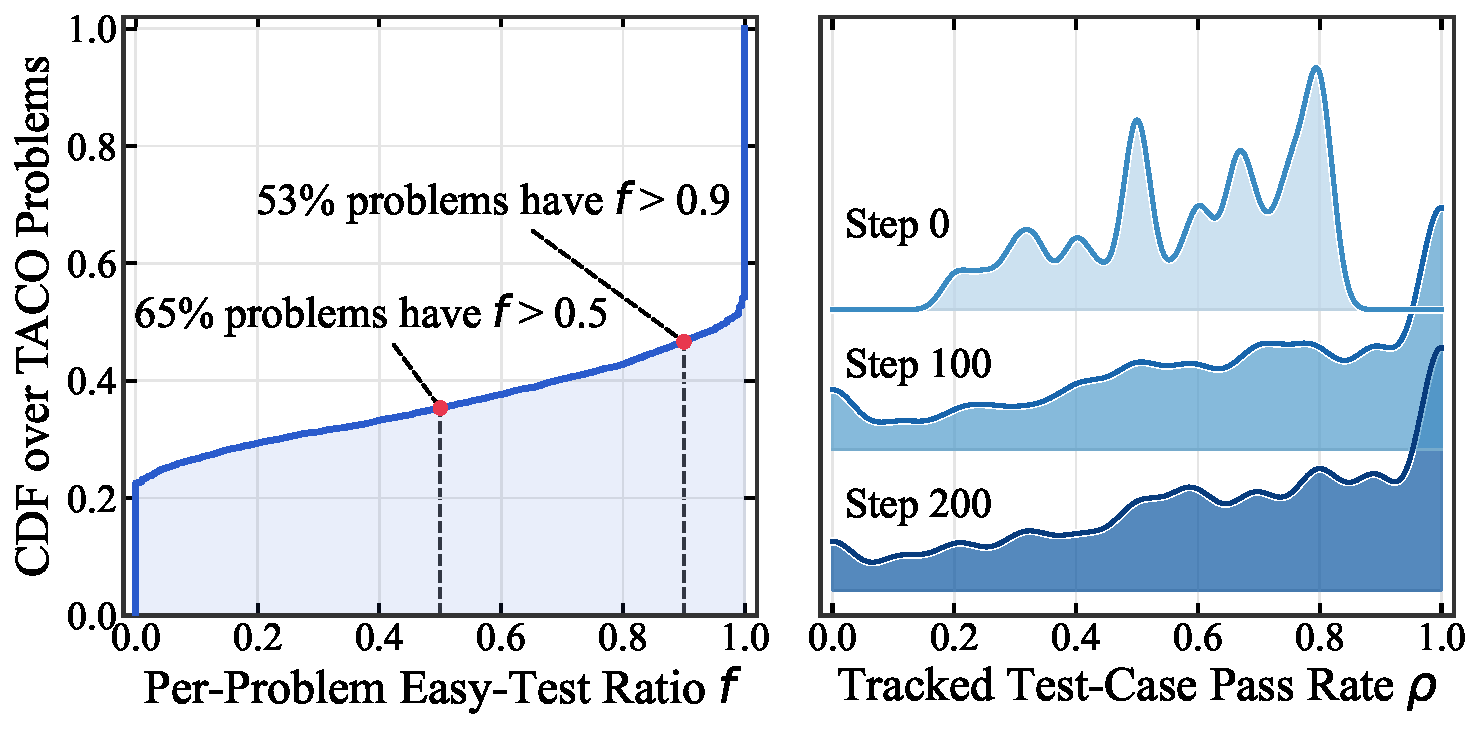
\includegraphics[width=0.8\textwidth]{paper_figure_taco.pdf}

\end{frame}

\begin{frame}{VeRPO: Turning Partial Success into Dense Rewards}

\textbf{Idea: combine two complementary signals}

\vspace{2mm}

\begin{columns}[t] % <-- key fix

\begin{column}{0.5\textwidth}
\raggedright % improves alignment consistency

\textbf{1. Local (dense signal)}

\begin{itemize}
    \item Use \textbf{test-case partial successes}
    \item Reward each step based on pass rate
    \item Captures fine-grained progress
\end{itemize}

\vspace{2mm}

\begin{flushleft}
\[
R^{turn}(\tau_i,t)
= \sum^{|U_x|}_{j=1} w'_j \cdot p^{(j)}_{t,i}
\]
\end{flushleft}

\end{column}

\begin{column}{0.5\textwidth}
\raggedright % same fix for symmetry

\textbf{2. Global (verifiable outcome)}

\begin{itemize}
    \item Final \textbf{pass/fail outcome}
    \item Down-weight long trajectories
    \item Ensures correctness signal
\end{itemize}

\vspace{2mm}

\begin{flushleft}
\[
\tilde{R}^{traj}
= R^{traj}(\tau_i)\cdot \gamma^{|\tau_i|}
\]
\end{flushleft}

\end{column}

\end{columns}

\end{frame}



\begin{frame}{VeRPO: Constructing Learning Signals}

\begin{columns}[b,onlytextwidth] % Changed alignment to bottom [b]

% ================= LEFT =================
\begin{column}{0.48\textwidth} % Reduced width slightly to prevent overflow

\textbf{Local (turn-level) signal}
\vspace{1mm}
\begin{itemize}
    \item Uses partial test-case success
    \item Provides step-level supervision
\end{itemize}

\vspace{2mm}

\begin{block}{Local advantage}
\vspace{-2mm}
\[
A^{\text{turn}}(\tau_i, t)
= R^{\text{turn}}(\tau_i, t)
- \operatorname{mean}(G(\mathcal{G}_x))
\]
\vspace{-4mm} % Adjusted to match right block spacing
\end{block}

\end{column}

\hfill % Ensures proper horizontal separation

% ================= RIGHT =================
\begin{column}{0.48\textwidth}
\vspace{0pt}

\textbf{Global (trajectory-level) signal}
\vspace{1mm}
\begin{itemize}
    \item Uses decayed outcome reward
    \item Captures overall correctness
\end{itemize}

\vspace{2mm}

\begin{block}{Global advantage}
\vspace{-2mm}
\[
A^{\text{traj}}(\tau_{i})
= \tilde{R}^{\text{traj}}(\tau_{i})
- \operatorname{mean}(\{\tilde{R}^{\text{traj}}(\tau_{j})\}_{j=1}^N)
\]
\vspace{-4mm}
\end{block}

\end{column}

\end{columns}

\end{frame}

\begin{frame}{VeRPO: Turn-Level Training Objective}

\textbf{Final step: combine global correctness with local progress}

\vspace{3mm}

\begin{block}{Turn-level advantage}
The trajectory-level signal is broadcast to each step and combined with the local advantage:
\end{block}

\vspace{-2mm}

\begin{equation}
A(\tau_i, t)
= A^{traj}(\tau_i)
+ \beta \cdot A^{turn}(\tau_i, t)
\end{equation}

\vspace{3mm}

\textbf{Interpretation}

\begin{itemize}
    \item $A^{traj}$ ensures global correctness (did the program solve the task?)
    \item $A^{turn}$ provides dense step-level credit assignment
    \item $\beta$ controls the trade-off between exploration and precision
\end{itemize}

\end{frame}

\begin{frame}[t]{Turning Partial Success into Dense Verifiable Rewards}
\small

\vspace{5mm}

\newcommand{\dashfill}{\leavevmode\cleaders\hbox to 0.5em{\hss-\hss}\hfill\kern0pt}

\centering
\setlength{\tabcolsep}{2.2pt}

\resizebox{\textwidth}{!}{%
  
\begin{tabular}{*{18}{c}}
\toprule
\multirow{3}{*}{Method} & \multirow{3}{*}{Train} & \multirow{3}{*}{RM} & \multirow{3}{*}{Reward} &
\multicolumn{4}{c}{HumanEval} &
\multicolumn{4}{c}{BigCodeBench} &
\multicolumn{2}{c}{LCB} &
\multicolumn{2}{c}{Codeforces} &
\multicolumn{2}{c}{Avg} \\

\cmidrule(lr){5-8} \cmidrule(lr){9-12} \cmidrule(lr){13-14} \cmidrule(lr){15-16}

& & & &
\multicolumn{2}{c}{-} & \multicolumn{2}{c}{Plus} &
\multicolumn{2}{c}{Full} & \multicolumn{2}{c}{Hard} &
\multicolumn{2}{c}{V6} & \multicolumn{2}{c}{CodeElo} &
\multicolumn{2}{c}{} \\

\cmidrule(lr){5-6} \cmidrule(lr){7-8} \cmidrule(lr){9-10}
\cmidrule(lr){11-12} \cmidrule(lr){13-14} \cmidrule(lr){15-16}
& & & & ST & MT & ST & MT & ST & MT & ST & MT & ST & MT & ST & MT & ST & MT \\

\midrule

Qwen3-8B & - & - & - &
91.03 & 95.05 & 87.49 & 90.14 & 35.85 & 58.32 & 16.38 & 41.69 &
27.12 & 28.14 & 20.77 & 22.73 & 46.44 & 56.01 \\

\midrule

\multirow{2}{*}{GRPO} & ST & - & 0-1 &
91.99 & 96.34 & 88.03 & 90.32 & \uline{36.33} & 57.87 & 16.87 & 40.54 &
28.35 & 29.28 & 28.49 & 30.72 & 48.34 & 57.51 \\

& MT & - & 0-1 &
91.46 & 96.41 & 87.57 & 91.23 & 35.73 & \uline{60.91} & 16.55 & \uline{43.32} &
28.35 & \uline{30.50} & 27.38 & 31.61 & 47.84 & \uline{59.00} \\

\addlinespace

\multirow{2}{*}{AceCoder} & ST & 7B & Dense &
\uline{92.04} & \uline{96.59} & \uline{88.71} & 91.46 & 36.07 & 58.36 &
14.86 & 39.53 & 27.78 & 27.57 & 25.06 & 26.96 & 47.42 & 56.74 \\

& MT & 7B & Dense &
\multicolumn{14}{c}{\dashfill Training Collapse \dashfill} \\

\addlinespace

\multirow{2}{*}{VeRPO} & ST & - & Dense &
\textbf{92.73} & 96.49 & \textbf{89.32} & \uline{91.84} &
\textbf{37.42} & 58.95 & \textbf{17.91} & 41.55 &
\textbf{29.72} & 30.14 & \textbf{30.50} & \uline{33.76} &
\textbf{49.60} & 58.79 \\

& MT & - & Dense &
91.69 & \textbf{97.87} & 88.05 & \textbf{93.14} &
36.10 & \textbf{62.52} & \uline{17.22} & \textbf{45.69} &
\uline{29.07} & \textbf{33.07} & \uline{29.03} & \textbf{40.44} &
\uline{48.53} & \textbf{62.12} \\

\bottomrule
\end{tabular}

}
\end{frame}

\begin{frame}{Beyond the 80/20 Rule}{High-entropy ``forking'' tokens}

\centering
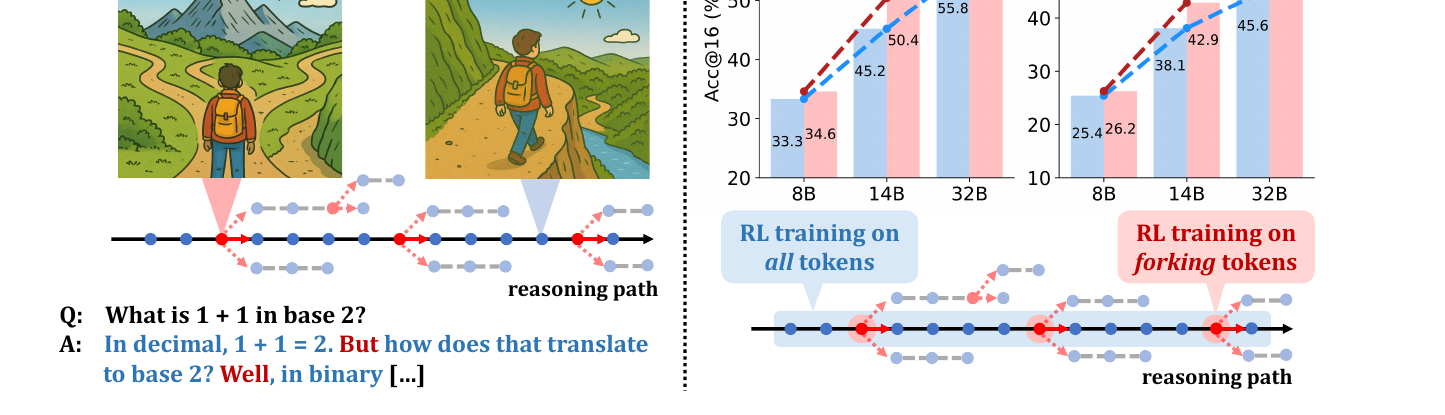
\includegraphics[width=0.95\textwidth,height=0.62\textheight,keepaspectratio]{forking_tokens_concept.png}

\begin{itemize}
    \item Only a \textbf{minority of CoT tokens are high-entropy} $\rightarrow$ they act as \emph{forks} that choose the reasoning path.
    \item RLVR training mostly adjusts exactly these high-entropy tokens.
\end{itemize}

\end{frame}

\begin{frame}{Beyond the 80/20 Rule}{20\% of tokens is enough}

\begin{columns}[c]

\begin{column}{0.46\textwidth}
\begin{itemize}
    \item Restrict policy-gradient updates to the top \textbf{20\% highest-entropy} tokens.
    \item Matches full-gradient training on Qwen3-8B and \textbf{beats} it at scale (32B: \textbf{+11.0} AIME'25).
    \item Training on the low-entropy 80\% instead \emph{hurts} performance.
\end{itemize}

\vspace{1mm}

\begin{block}{Takeaway}
The learning signal is concentrated in a sparse set of decisive tokens.
\end{block}
\end{column}

\begin{column}{0.54\textwidth}
\centering
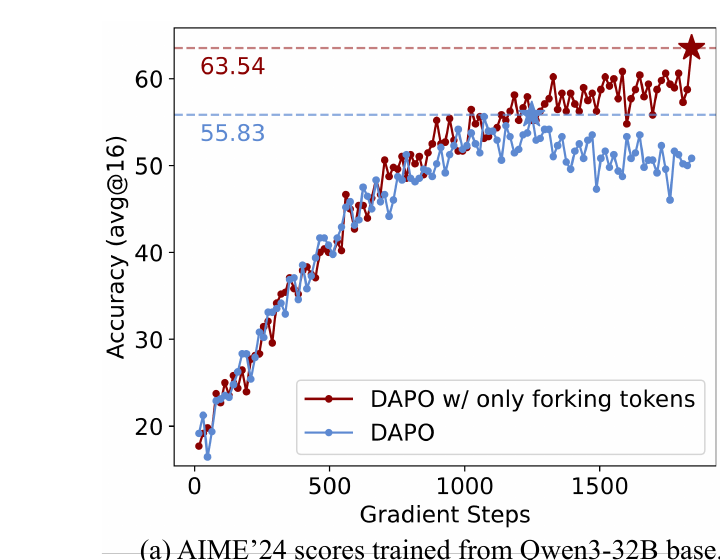
\includegraphics[width=\textwidth,height=0.78\textheight,keepaspectratio]{forking_tokens_results.png}
\end{column}

\end{columns}

\end{frame}

\begin{frame}{TIP: Token Importance in On-Policy Distillation}{The idea}

\centering

\begin{tikzpicture}[
    font=\small,
    tok/.style={draw, rounded corners, minimum width=1.2cm, minimum height=0.7cm},
    teacher/.style={tok, fill=TUMBlue!25},
    student/.style={tok, fill=TUMBlue!8},
    crit/.style={tok, fill=TUMOrange!30, very thick},
    flow/.style={->, thick, TUMBlue},
    div/.style={<->, thick, TUMOrange},
]

% --- Teacher track (top): provides target distribution ---
\node[align=center, font=\bfseries] (tlab) at (-0.2, 0.95) {Teacher\\[-1pt]\scriptsize strong};
\node[teacher, right=1.1cm of tlab] (t1) {$q_1$};
\node[teacher, right=0.45cm of t1]  (t2) {$q_2$};
\node[teacher, right=0.45cm of t2]  (t3) {$q_3$};
\node[teacher, right=0.45cm of t3]  (t4) {$q_4$};
\node[TUMBlue, font=\scriptsize] at ($(t1)!0.5!(t4) + (0,0.56)$) {provides target distribution};

% --- Student track (bottom): generates rollout on-policy ---
\node[align=center, font=\bfseries] (slab) at (-0.2, -0.95) {Student\\[-1pt]\scriptsize weak};
\node[student] (s1) at (t1 |- slab) {$x_1$};
\node[student] (s2) at (t2 |- slab) {$x_2$};
\node[crit]    (s3) at (t3 |- slab) {$x_3$};
\node[student] (s4) at (t4 |- slab) {$x_4$};

\draw[flow] (s1) -- (s2);
\draw[flow] (s2) -- (s3);
\draw[flow] (s3) -- (s4);
\node[font=\scriptsize] at ($(s1)!0.5!(s4) + (0,-0.56)$) {generates rollout (on-policy)};

% --- Divergence between the tracks ---
\draw[div] (t1) -- (s1) node[midway, right, font=\scriptsize] {$\delta_1$};
\draw[div] (t2) -- (s2) node[midway, right, font=\scriptsize] {$\delta_2$};
\draw[div, line width=1.4pt] (t3) -- (s3)
    node[midway, right, font=\scriptsize\bfseries, TUMOrange] {$\delta_3$ large};
\draw[div] (t4) -- (s4) node[midway, right, font=\scriptsize] {$\delta_4$};

\node[align=center, font=\scriptsize, TUMOrange, right=0.3cm of s4, xshift=0.2cm]
    {important\\token};

\end{tikzpicture}

\vspace{2mm}

\begin{block}{Token importance}
Combine student uncertainty $h_t$ and divergence $\delta_t$ \;$\Rightarrow$\; distill the tokens carrying knowledge the student lacks.
\end{block}

\end{frame}

\begin{frame}{TIP: Token Importance in On-Policy Distillation}{Which tokens carry the signal?}

\centering
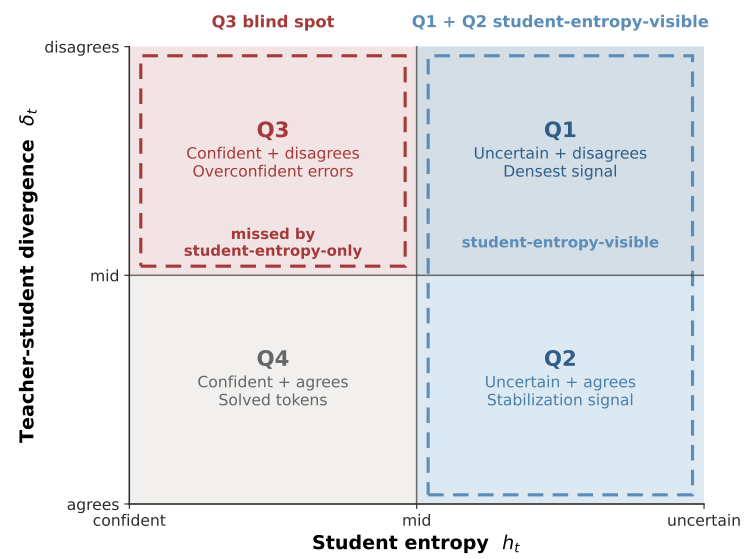
\includegraphics[width=0.72\textwidth,height=0.74\textheight,keepaspectratio]{token_quadrants.png}

\end{frame}

\begin{frame}{TIP: Token Importance in On-Policy Distillation}{Results:}

\centering
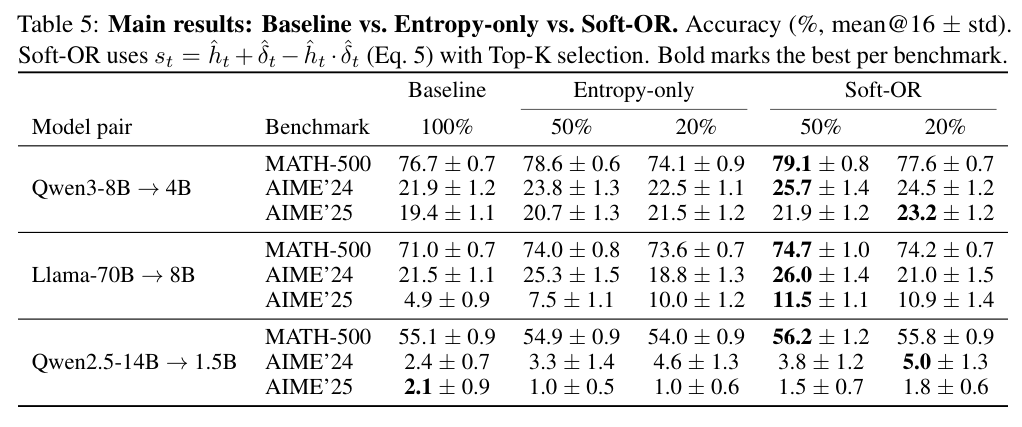
\includegraphics[width=0.95\textwidth]{results.png}

\end{frame}

% --- PRIME: Motivation ---

\begin{frame}[t]{PRIME: Process Reinforcement through Implicit Rewards}{Motivation}
\footnotesize

\begin{columns}[T,onlytextwidth]

\begin{column}{0.47\textwidth}
\textbf{Problem}

\vspace{1mm}

\begin{itemize}
  \setlength\itemsep{3pt}
  \item Outcome rewards are sparse: only the final answer is scored.
  \item Process rewards would give denser credit assignment.
  \item But standard PRMs need step labels, online updates, and extra training.
\end{itemize}

\vspace{2mm}

\textbf{PRIME's goal}

\vspace{1mm}

\begin{itemize}
  \setlength\itemsep{3pt}
  \item Get dense token-level rewards.
  \item Use only outcome labels.
  \item Avoid a separate PRM training stage.
\end{itemize}

\end{column}

\begin{column}{0.51\textwidth}
\centering
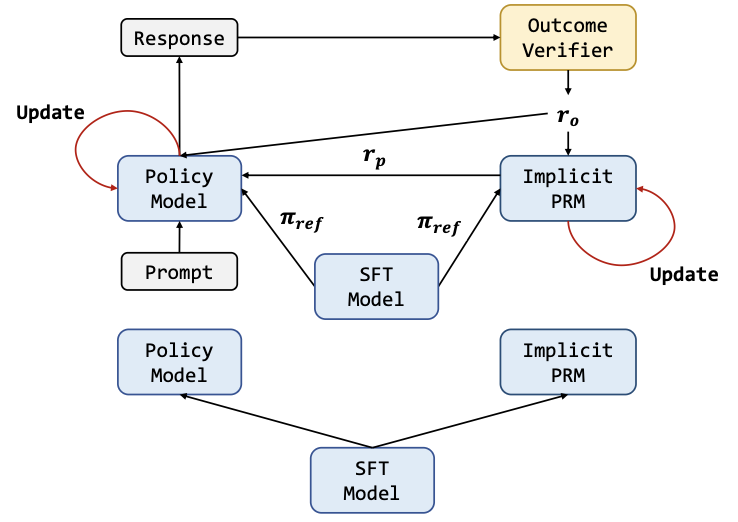
\includegraphics[
  width=\textwidth,
  height=0.62\textheight,
  keepaspectratio
]{prime_fig1.png}

\vspace{1mm}
{\scriptsize
\textbf{Figure 1.} PRIME initializes the policy and implicit PRM from the same SFT model, then updates both online using outcome labels.
}
\end{column}

\end{columns}

\end{frame}


% --- PRIME: Key Idea ---

\begin{frame}[t]{PRIME: Process Reinforcement through Implicit Rewards}{Implicit Process Rewards}
\footnotesize

\textbf{Core idea:} train an ORM so it can also act as a PRM at inference time.

\vspace{3mm}

\[
  r_\phi(y_t)
  =
  \beta \log
  \frac{\pi_\phi(y_t \mid y_{<t})}
       {\pi_\text{ref}(y_t \mid y_{<t})}
\]

\vspace{1mm}

\begin{itemize}
  \setlength\itemsep{4pt}
  \item Reward is a \textbf{log-ratio} between a learned model and a reference.
  \item This gives a \textbf{dense token-level signal}.
  \item Training still uses only \textbf{binary outcome labels}.
  \item Online updates reduce distribution shift and reward hacking.
\end{itemize}

\vspace{2mm}

\begin{center}
\textbf{Takeaway:} dense process supervision without manually labeled steps.
\end{center}

\end{frame}


% --- PRIME: Training Signal ---

\begin{frame}[t]{PRIME: Process Reinforcement through Implicit Rewards}{Training Signal}
\footnotesize

\textbf{PRIME combines two reward sources:}

\vspace{3mm}

\[
A_t
=
\underbrace{A_t^{\text{process}}}_{\text{dense token-level signal}}
+
\underbrace{A^{\text{outcome}}}_{\text{final correctness signal}}
\]

\vspace{4mm}

\begin{itemize}
  \setlength\itemsep{5pt}
  \item \textbf{Process term:} assigns credit across reasoning tokens.
  \item \textbf{Outcome term:} keeps optimization tied to final correctness.
  \item Both terms use RLOO-style normalization across rollouts.
\end{itemize}

\vspace{3mm}

\begin{center}
\textbf{Why it matters:} PRIME keeps the reliability of verifiable rewards while making them denser.
\end{center}

\end{frame}


% --- PRIME: Results ---

\begin{frame}[t]{PRIME: Process Reinforcement through Implicit Rewards}{Results}
\footnotesize

\begin{columns}[T,onlytextwidth]

\begin{column}{0.52\textwidth}
\centering
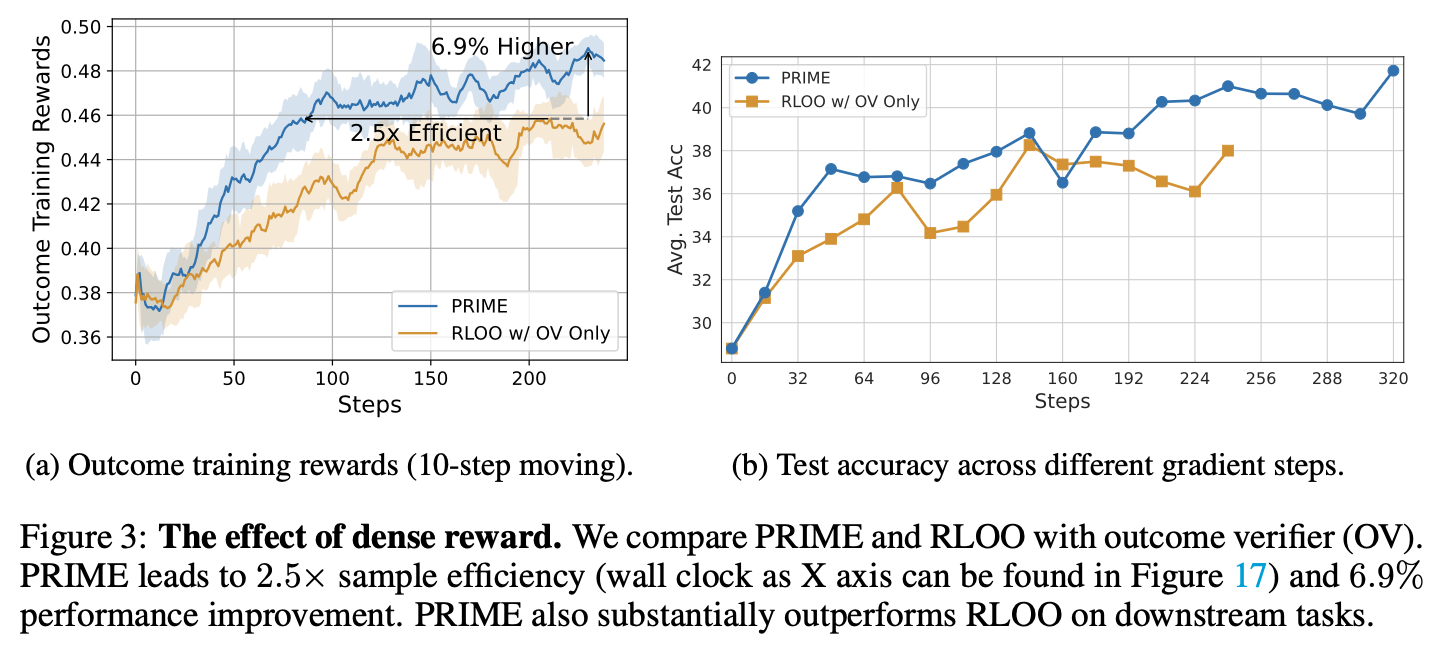
\includegraphics[
  width=\textwidth,
  height=0.66\textheight,
  keepaspectratio
]{prime_fig3.png}
\end{column}

\begin{column}{0.46\textwidth}
\centering
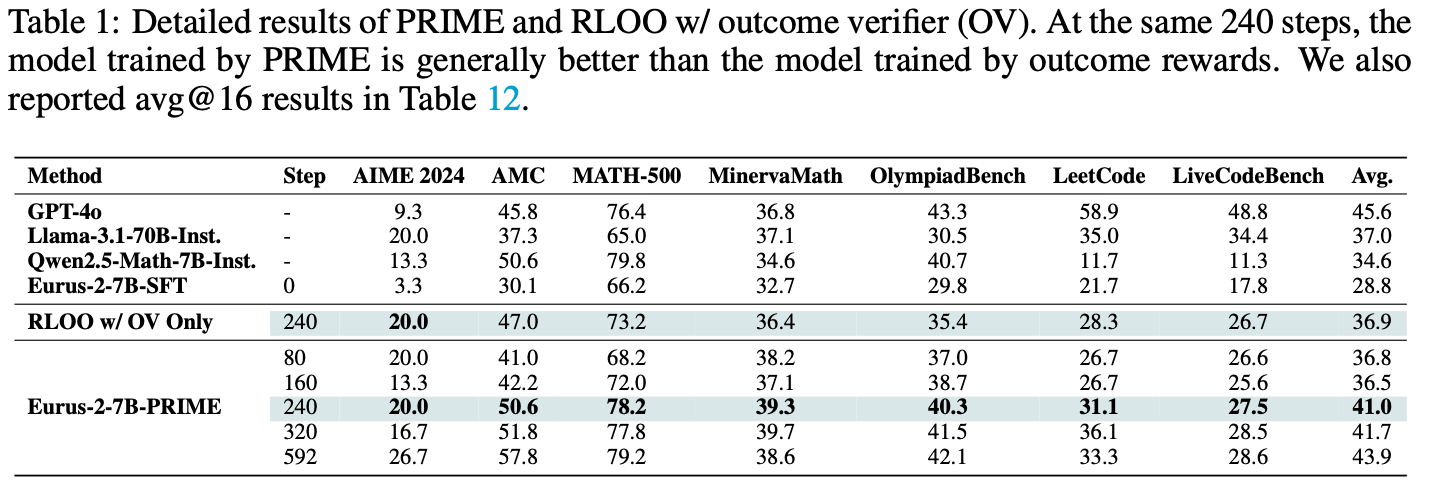
\includegraphics[
  width=\textwidth,
  height=0.66\textheight,
  keepaspectratio
]{prime_table1.png}
\end{column}

\end{columns}

\vspace{2mm}

\begin{center}
\textbf{Key result:} PRIME is more sample-efficient than outcome-only RL and improves the SFT baseline substantially.
\end{center}

\end{frame}

\section{Progress}

% ===================== Journey timeline =====================
\begin{frame}{Progress}{From toy matrices to a 4B model}

\centering
\vspace{2mm}

\begin{tikzpicture}[
    every node/.style={font=\small},
    milestone/.style={
        draw, rounded corners, align=center,
        minimum height=1.5cm, text width=2.5cm,
        fill=TUMBlue!10
    },
    current/.style={
        draw, rounded corners, align=center,
        minimum height=1.5cm, text width=2.5cm,
        fill=TUMBlue!30, very thick
    }
]

\node[milestone] (m1) {\textbf{Toy matrices}\\\scriptsize MNIST-scale MLPs};
\node[milestone, right=0.9cm of m1] (m2) {\textbf{Small GPT-2}\\\scriptsize first real LM};
\node[milestone, right=0.9cm of m2] (m3) {\textbf{Qwen3.5-0.8B}\\\scriptsize scaling up};
\node[current,   right=0.9cm of m3] (m4) {\textbf{Qwen3.5-4B}\\\scriptsize current focus};

\draw[->, very thick, TUMBlue] (m1) -- (m2);
\draw[->, very thick, TUMBlue] (m2) -- (m3);
\draw[->, very thick, TUMBlue] (m3) -- (m4);

\node[above=1mm of m4, font=\footnotesize\bfseries, TUMBlue] {you are here};

\end{tikzpicture}

\vspace{4mm}

\begin{itemize}
    \item Built on existing tensor-disentanglement code; first validated the effect on tiny weight matrices.
    \item Scaled progressively to confirm the approach holds on real language models.
\end{itemize}

\vfill
{\scriptsize Based on ongoing work by our supervisor Tristan Till (sebis, TUM).}

\end{frame}

% ===================== Disentanglement engineering + LR sweep =====================
\begin{frame}{Progress}{Tuning the disentanglement}

\begin{columns}[c]

\begin{column}{0.42\textwidth}
\begin{itemize}
    \item Performance optimizations for scale.
    \item Learning-rate sweep for stability.
\end{itemize}

\vspace{2mm}

\begin{block}{Takeaway}
Large rates diverge; a mid-range rate minimizes both cost and effective rank.
\end{block}
\end{column}

\begin{column}{0.58\textwidth}
\centering
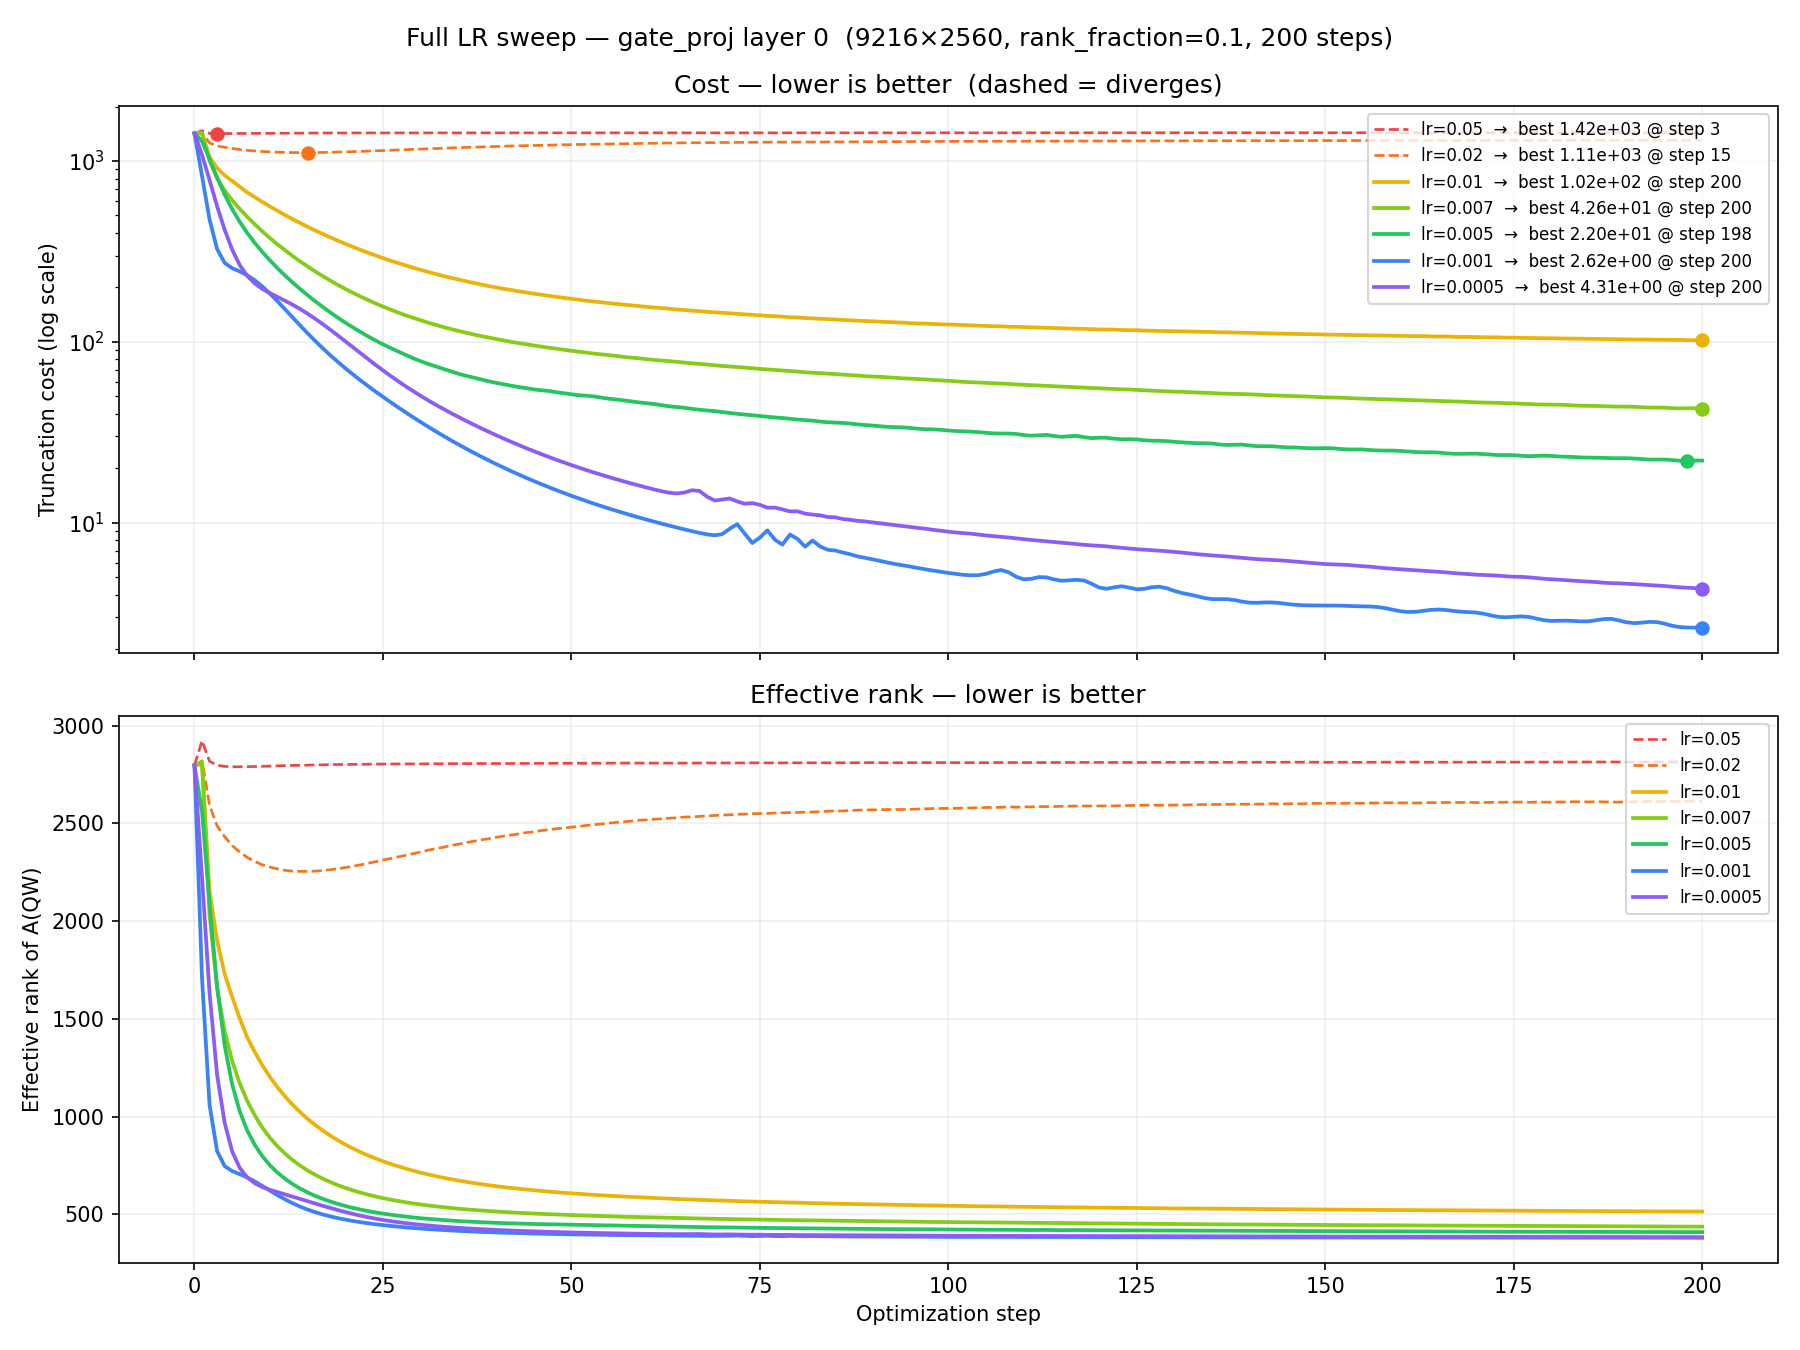
\includegraphics[width=\textwidth,height=0.72\textheight,keepaspectratio]{lr_sweep.png}
\end{column}

\end{columns}

\end{frame}

% ===================== MMLU vs rank =====================
\begin{frame}{Progress}{Quality vs.\ compression}

\centering
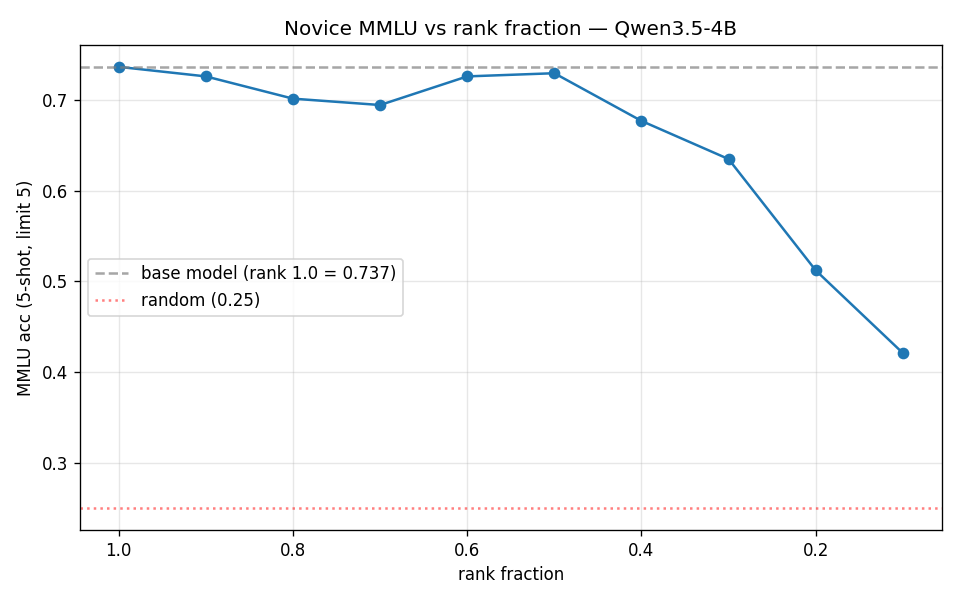
\includegraphics[width=0.55\textwidth,height=0.5\textheight,keepaspectratio]{mmlu_rank_sweep.png}

\begin{itemize}
    \item MMLU accuracy holds near the base model down to rank fraction $\approx 0.5$.
    \item Below that, quality drops sharply --- the Novice becomes degenerate near rank $0.1$.
    \item Gives us a controllable knob for how much weaker the Novice should be.
\end{itemize}

\end{frame}

\section{Outlook}

\begin{frame}{Outlook}{Next steps}

\begin{itemize}
    \item Run experiments with the \textbf{Qwen3.5-4B} model, generating rollouts on a \textbf{math reasoning dataset}.
    \item \textbf{Quantitative \& qualitative evaluation} of which specific tokens drive divergence between the Master and the Novice.
    \item Explore how to \textbf{integrate this signal into a reinforcement learning setup}.
\end{itemize}

\vspace{4mm}
\centering
\begin{tikzpicture}[every node/.style={font=\footnotesize}]
    \node[draw, rounded corners, fill=TUMBlue!30, minimum height=0.9cm, text width=2.6cm, align=center] (now) {\textbf{Qwen3.5-4B}\\disentangled};
    \node[draw, rounded corners, dashed, minimum height=0.9cm, text width=2.6cm, align=center, right=0.8cm of now] (roll) {Master/Novice\\rollouts};
    \node[draw, rounded corners, dashed, minimum height=0.9cm, text width=2.6cm, align=center, right=0.8cm of roll] (tok) {Token-level\\divergence analysis};
    \node[draw, rounded corners, dashed, minimum height=0.9cm, text width=2.6cm, align=center, right=0.8cm of tok] (rl) {RL\\integration};

    \draw[->, very thick, TUMBlue] (now) -- (roll);
    \draw[->, very thick, TUMBlue, dashed] (roll) -- (tok);
    \draw[->, very thick, TUMBlue, dashed] (tok) -- (rl);
\end{tikzpicture}

\end{frame}

\section{References}

\begin{frame}{References}

\small

\begin{itemize}
    \item Longwen Wang et al. (2026).
    \textit{Beyond Binary: Turning Partial Success into Dense Verifiable Rewards for Reinforcement Learning in Code Generation}.
    arXiv:2601.03525
    \item Yuanda Xu et al. (2026).
    \textit{TIP: Token Importance in On-Policy Distillation}.
    arXiv:2604.14084
    \item Shenzhi Wang et al. (2025).
    \textit{Beyond the 80/20 Rule: High-Entropy Minority Tokens Drive Effective Reinforcement Learning for LLM Reasoning}.
    arXiv:2506.01939
    \item Ganqu Cui et al. (2025).
    \textit{Process Reinforcement through Implicit Rewards}.
    arXiv:2502.01456
\end{itemize}

\end{frame}

\end{document}
